\svnkwsave{$RepoFile: elton/blog/AdamBlog.tex $}
\svnidlong {$HeadURL: svn://zero.physics.gatech.edu/elton/blog/AdamBlog.tex $}
{$LastChangedDate: 2022-08-18 21:48:08 -0400 (Thu, 18 Aug 2022) $}
{$LastChangedRevision: 550 $} {$LastChangedBy: predrag $}
\svnid{$Id: AdamBlog.tex 550 2022-08-19 01:48:08Z predrag $}

  \renewcommand{\ssp}{x}            %state space point

\chapter{Adam's research blog}
% on Lagrangian mixing}
\label{chap:AdamBlog}

Adam Fox unpublished recalculation of Lan's\rf{LCC06} invariant torus.

\input FoxCvi14flotsam

    \section{Daily blog}
    \label{sect:DailyAdam}


\bigskip

\noindent
{\color{red} The latest entry at the bottom for this part of the blog}
$\footnotemark\footnotetext{{\tt \svnkw{RepoFile}}, rev. \svnfilerev:
 last edit by \svnFullAuthor{\svnfileauthor},
 \svnfilemonth/\svnfileday/\svnfileyear}$
\bigskip\bigskip


\begin{description}

\AFpost{2013-11-11}{
Title: Computation of quasiperiodic solutions to the Kuramoto-Sivashinsky
Equation
    }

    \PCpost{2013-08-26}{
I see an orgy of invariant tori in your future, the full, exact
Navier-Stokes, not a model of anything. Here, in Elton's blog, is what we
have so far - you can take that ball and run with it, and it will be
really easy to get started. Turns out equilibria of shear flows are
really bad mixers - but the \po s might do a better job
    }

\AFpost{2013-08-29}{
I had a great meeting with Cristel on Wednesday.  He gave me a lot to
think about with regards to developing some renormalization theory for
volume-preserving systems.

I've been reading through the notes you sent me, and I've started working
through some books on Navier-Stokes as well.  I'm excited to jump into
this work.

From your letter it seems that my first goal should be to study the
mixing in periodic flows.  Ideally, I'd be able to move on and compute
quasi-\po s and study the mixing there as well.  Does that seem
reasonable?

Finally-is there a ``standard" measure of mixing that you use?  It seems
there are many ways we could measure this, but I thought you might have
some preferences.
    }

 \PCpost{2013-08-30}{
Think thrice before plunging into renormalization theory :)

I've scribbled a few mixing ideas in the Elton blog, but no - I'm open to any
reasonable measure of mixing. Eventually, what you want to develop is a
theory of 3D turbulent diffusion, computable from a set of invariant
solutions of the exact Navier-Stokes - I think you will need \po s and
\rpo s, \eqva\ are only a warm-up.
    }

\AFpost{2013-09-12}{
    Do you have any notes on your previous students' work computing tori?
    That might be a good place for me to start.
    }

\PCpost{2013-09-12}{
Your problem is easier, as for equilibria you would be computing tori in
3D incompressible flow with plane Couette symmetries.

There are two more repositories - but for starters, see
the families of two-dimensional tori in 5 dimensional phase space
example, \emph{Sect B. Lower dimensional invariant tori}, in
Pa\v{s}kauskas, Chandre, and Uzer\rf{paskauskas2009a}.

In $\infty$-dimensions Lan computes tori for \KS,
see Lan and C. Chandre and P. Cvitanovi\'{c}\rf{LCC06}
\emph{Variational method for locating invariant tori}.

`Newton descent' is explained in \refref{CvitLanCrete02,lanVar1}. I'm
sure you, Jim and Rafael know how to compute these much better than what
Lan, Cristel, Rytis and I knew 8 years ago...
    }

\PCpost{2013-09-19 to Burak}{
Please go to Adam Kamor (he's here right now) and learn how to use his
unstable manifold Poincar\'e sections code - looks very smart (Adam Fox
approved), then put a copy of the code into the repository.
I do think you also want to get the code from him - looks very good, and
applicable to our unstable manifolds, Poincar\'e return maps.
Interpolation is cubic splines. There must be some good algorithm to also
compute curvilinear distance from cubic splines?
It should
help you get the return maps for the 2-mode problem, and it should become
very useful once we symmetry reduce KS flow (and NS! :)
\\
{\bf Burak}:
I met Adam yesterday, he explained me his algorithm, showed results and
passed me the reference paper.
    }

\AFpost{2013-09-23}{
I'm working on Lan's code for the standard map.  I believe that I have it
working, however it is very slow (granted, I'm integrating the ODEs in a
very stupid way, but still).

I couldn't find any specific references to convergence speed, runtime, or
anything else.  Do you happen to know what Lan's typical runtime was?
    }

\YLpost{2013-09-29}{
As far as I can recall, the computation is not as fast as the cycle
searching program but it is not extremely slow. The main problem is not
the speed but the set-up of initial conditions. If the initial condition
is not good, then it does not converge at all. Such a problem exists even
for the cycle searching program but the constraint is not so stringent.
The runtime of course depends on the problem itself, how the program is
written and parameter values.  For the standard map, it takes a couple of
minutes if several hundred lattice points are used. The acceleration
scheme is described in the cycle searching paper.
    }

\AFpost{2013-10-01}{
I've got the code up and working well - for the standard map at least.  I
wanted to chat with you a little bit before starting the far more
complicated task of computing tori in the Couette system.
    }

\PCpost{2013-09-12}{
You might want the full subversion repository, with John's programs, etc.
Get through the GaTech firewall using  \texttt{anyc.vpn.gatech.edu}, then

svn co svn://zero.physics.gatech.edu/elton
\\
          afox33  wet\&wild

(I'm assuming you know how to use subversion on linux, tortoiseSVN on
MSwindows, or like)
    }


   \PCpost{2013-10-03}{
Added Greg Byrne and Adam Fox to the repo.
    }

\AFpost{2013-10-13}{
I've finished the code to compute tori in the \KS\
system.  I'm still a bit unsure how to generate a good guess for the
initial condition.  Do you recall the values you used in your paper, or
how you generated them?  Any suggestions for a good place to start?
    }


    \PCpost{2013-10-03}{
Lan's files are in \texttt{elton/y-lan/papers/kuramot/}, see
\texttt{elton/00ReadMe.txt} for details (also my email of 2013-10-16. I
have tried to upload all files called by \texttt{torusmake} and
\texttt{torusorb.f}, if I have missed some, let me know which ones do you
need.

\texttt{torusorb.f} inputs \texttt{torusks412b.dat}, but that's an
empty file. You probably want to uncomment \texttt{torusks412a.dat}
instead.
    }

\AFpost{2013-08-29 to Lan}{
I'm looking at the data now but am unsure what I'm looking at.  The file
'\texttt{torusks412a}' contains an array of length 2049.  I'm guessing that I
should interpret it as a 16x128 matrix (with some random extra point that
doesn't fit in-i'll ignore that).  Is that correct?  So these are 16
fourier modes of the KS system, with 128 points on the Poincar\'e
section?
    }

    \PCpost{2013-10-03}{
Probably not a good idea, but here is what I have been thinking. When
you have an exact continuous symmetry - let's say \SOn{2} - then a
\rpo\ fills out ergodically a torus. The Floquet matrix evaluated for
a one period at a torus point $\ssp$ has two unit multipliers, one
along the velocity tangent $\vel(\ssp)$, and the other along the
group tangent $\groupTan(\ssp)$. It is sufficient to specify just one
point $\ssp$ in the invariant torus, the rest is given by the
integration over the two tangent fields; as they commute, it is just
one integral in time direction by $\period{p}$, and one $\SOn{2}$
rotation by $\shift_p$.

Can we do the same for the invariant torus you are computing? One
direction is the velocity field $\vel(\ssp)$, but I am not sure how
we define and integrate the other tangent field, and when do we get
unit multipliers...
    }

\AFpost{2013-11-01}{
I think I have the variational method working for \KS. What do we want to
look at.  I have a few ideas, but I'm sure you do too.
    }

\AFpost{2013-11-09}{
This code still isn't working quite right and I'm not sure what the
problem is, although I think it may be an issue with the {\jacobianM}.

If we take a Poincar\'e section at $a_1=0.06$, and compute the {\jacobianM} for
the Poincar\'e map, am I correct in thinking that the first row should be
zeros?  Since $a_1$ does not change, it seems natural that all the
derivatives,  $d a_1 / d a_j  = d (const) / d a_j$, should be zero.
Is that correct?
    }

\AFpost{2013-11-14}{
I am having trouble getting this code to work - I really have no idea
what the problem is.  It's essentially the same code I used for the
standard map, but with a small modification.

%%%%%%%%%%%%%%%%%%%%%%%%%%%%%%%%%%%%%%%%%%%%%%%
\SFIG{131114JacobianKS}{}{
A first \KS\ Fourier mode, and the first entry in the {\jacobianM}.
}{fig:131114JacobianKS}
%%%%%%%%%%%%%%%%%%%%%%%%%%%%%%%%%%%%%%%%%%%%%%%

The only issue I can think of is that I'm integrating the {\jacobianM}
incorrectly.  The values do seem to be pretty large - see
\reffig{fig:131114JacobianKS} as an example.  The {\jacobianM} changes much
more significantly than the state variables.  Do you know if this is
typical?  Are there are ways you can think of for me to test my code?
Any standard examples or anything?
    }

\PCpost{2013-11-14}{
{\JacobianM} elements typically grow exponentially with time. But here
it is hard to tell, perhaps the time is short. Does not look particularly
suspicious.

I would test the code on a \rpo\ - that is a torus in
the full state space, a torus that we know \emph{exactly}, to arbitrary
precision, so initial guess will be very easy... The easiest example
is the one Burak is working on
Porter and Knobloch\rf{PoKno05}
2-Fourier modes 'truncation of a PDE'
which is 4 dimensional:
\bea
\dot{x}_1 &=& (\mu_1 + a_1 r_1^2 + b_1 r_2^2 + c_1 x_2)x_1 + c_1 y_1 y_2 + e_1 y_1
\continue
\dot{y}_1 &=& (\mu_1 + a_1 r_1^2 + b_1 r_2^2 - c_1 x_2)y_1 + c_1 x_1 y_2 - e_1 x_1
\continue
\dot{x}_2 &=& (\mu_2 + a_2 r_1^2 + b_2 r_2^2)x_2 + c_2 (x_1^2 - y_1^2) + e_2 y_2
\continue
\dot{y}_2 &=& (\mu_2 + a_2 r_1^2 + b_2 r_2^2)y_2 + 2 c_2 x_1 y_1 - e_2 x_2
\continue
		  && \mbox{where } r_1^2 = x_1^2 + y_1^2\, , \quad r_2^2 = x_2^2 + y_2^2
\,.
\label{2mode4D}
\eea
Burak can give you the parameter values and the initial point for ten or
so \rpo s. \refFig{fig:BBO2RpoSspComovSlice} illustrates the 2D torus
embedded in 4D that
your code should absolutely be able to find.

\begin{figure}%[H]
\centering
 (a) 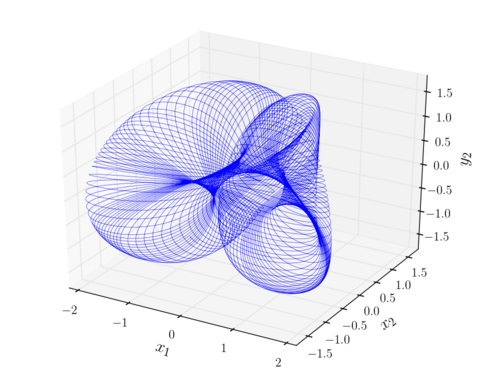
\includegraphics[width=0.45\textwidth]{BBO2a1045rpossp}
 (b) 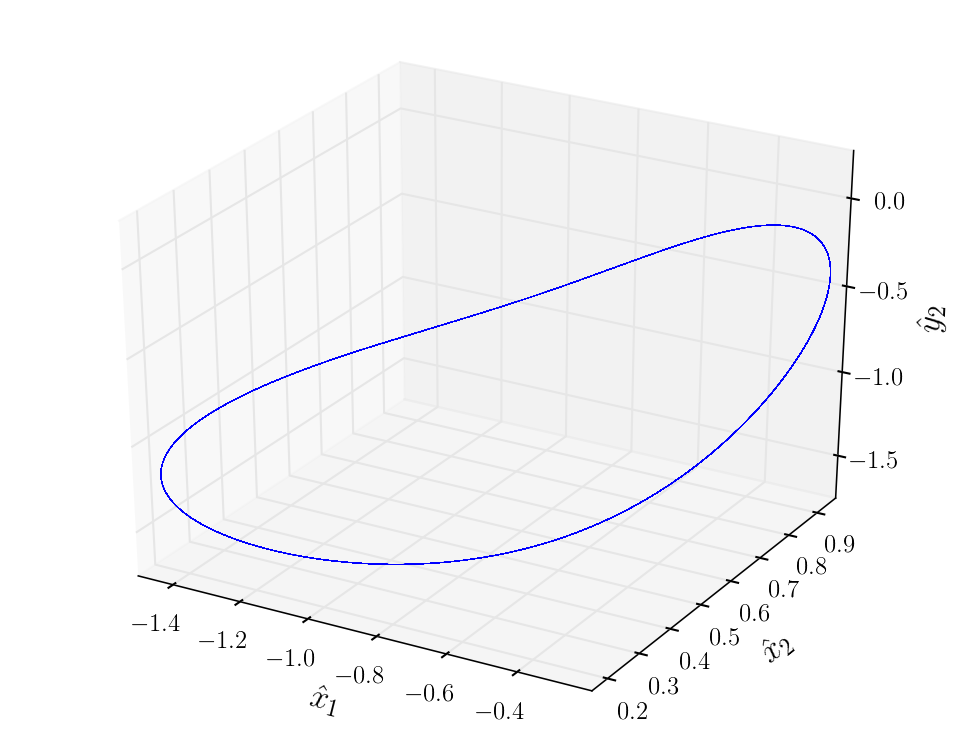
\includegraphics[width=0.45\textwidth]{BBO2a1045rposlice}
\caption{
(a)
\Rpo\ \cycle{01} integrated for a number of periods $\period{01}$. It
explores ergodically the group orbit of the \rpo, a $2D$ invariant
torus embedded in $4D$.
This is a $3D$ projection of the
full $4D$ \statesp\ \On{2}-equivariant {\twoMode} flow
\refeq{2mode4D}.
Other projections on any three coordinates
$\{x_1,y_1,x_2,y_2\}$ are qualitatively similar.
(b) In the \slice\ this trajectory retraces the corresponding \po.
}
\label{fig:BBO2RpoSspComovSlice}
\end{figure}

The next example would be a short \rpo\ in \KS, but in
the full state space, not the subspace you are working in. We have
60,000 of those :)
    }

\PCpost{2013-11-18}{
The 2 mode model of Burak's
\HREF{http://chaosbook.org/~predrag/old/2modes.pdf}{2modes.pdf} is a
perfect test for your tori-searching routines; the relative orbit 01
given by the diagonal crossing in ref fig. 46 on p. 76  (for example)
fills out a torus in 4-dimensions; your routines should find it. You have
an arbitrarily precise initial guess: it is the group orbit of the fixed
point on the diagonal, one of the 'baseball' seams in fig. 63 on p. 89.
    }

\AFpost{2013-11-22}{
I've been working on finding tori in Lan's\rf{LCC06} 1.5 DOF Hamiltonian.  Recall
that I was able to compute a torus, but it was ``boring" - basically it
looked purely sinusoidal.  It also appeared to be more robust than the
torus Lan had in the paper.

I haven't been able to find anything wrong with my work, so I tried
something different - I computed the Golden Mean torus rather than golden
mean - 1 (which Lan used in the paper) torus.  This had a big effect -
the torus now has the irregular shape that I would expect, and looks
similar to the torus in the paper (although up-side down and stretched)

I wonder if perhaps Lan's figures are for some other rotation number?  Or
maybe he exploited some symmetry relations?  Do you have any thoughts?
    }

\AFpost{2013-11-23}{
When I integrate to get the \jacobianM\ in \KS, I find the
determinant goes to zero very rapidly.

Is this something we would expect?
    }

\PCpost{2013-11-23}{
yes, it has very strongly contracting stability multipliers (contracting
as $\exp(-t k^{-4})$). Xiong Ding is evaluating them accurately as his
project, but I do not think it is important for you (as yet :) - for
Newton you need the expanding multipliers, and a set of the least
contracting multiplier.
    }

\AFpost{2013-11-26}{
Is there anything special about the 5th Fourier mode in \KS?

If I remove this mode from my algorithm, then I can get it to converge
perfectly (as in, I hold this mode constant, and ignore its contribution
to the error).
    }

\PCpost{2013-12-01}{
that's super weird. No clue... When you look at the winding number, are
you close to m/5 resonance?
    }

\AFpost{2013-12-02}{
That's a good thought-I'm using the golden mean and 5 is a Fibonnaci
number, but I doubt that's the problem.

The good news is that my code is working for the periodically forced
Hamiltonian.

So I'm convinced the problem is numerical-maybe aliasing or something
similar?  I'm optimistic that I'll have good results by Dynamics Days.
    }

\AFpost{2013-12-05}{
I figured out why the algorithm appeared to converge for very large L.
I'm still pretty stumped overall though.  I'm going to quickly try to
compute the `islands' in the standard map - all the tori I've computed so
far have been rotational.  Maybe there is some trick for the
non-rotational tori?

Also- we are using $a_1 = 0.06$ as a Poincar\'e section.  Should I ``ignore"
that section in the process?  As in-should the {\jacobianM} really be
15x15 rather than 16x16 (since the first mode is fixed?)

I think I'll start working on the \twoMode\ system described above,
see {\bf [Predrag 2013-11-14]}.
    }

\PCpost{2013-12-05}{
We are using $a_1 = 0.06$ as a Poincar\'e section. The {\jacobianM}
of the return map is 15x15. If you instead compute the continuous
time {\jacobianM}, that is 16x16, with one multiplier 1 (to your numerical precision).
Read
\HREF{http://www.streamsound.dk/book1/chaos/chaos.html\#104/z} {this}.
    }

\PCpost{2013-12-05}{
Lange~\etal\rf{LROBK13}
{\em Global structure of regular tori in a generic 4D symplectic map}
might be of interest to Adam.
    }

\AFpost{2013-12-16}{\KS\ {\JacobianM} issues: in one
paper they reference the ``back-flying" time (?)
\\
{\bf Predrag}
Google finds it only in Lan's
\HREF{http://www.cns.gatech.edu/~y-lan/thesis/thesis.pdf}
{thesis}\rf{Lan:Thesis}, p.96.
It is a discussion about how to find the eigenvectors within the
Poincar\'e section. ``Back-flying" is probably Lan's word for the small
time adjustment needed for a neighboring trajectory to land in the
Poincar\'e section. This discussion is related to your question whether one
simply sets a column and a row in the {\jacobianM} to zero (I think not).

We also discuss the relation of the full space {\jacobianM} and
Poincar\'e section {\jacobianM}
\HREF{http://www.streamsound.dk/book1/chaos/chaos.html\#104/z}{here}. If
anyone has a simpler, more elegant synthesis/rewrite, I would dearly like
to include it in the ChaosBook.

PS to others: Adam's invariant tori searches are working for several
simpler models, but seem not to work for \KS. Suspicion
is that he is not coding the Poincar\'e section {\jacobianM} correctly - that's
why I'm copying you on this email.
 }
\AFpost{2013-12-14}{
Added \refsect{sect:ToriVariational}.
}

\AFpost{2013-12-16}{
OK-still working on the \KSe.  The problem, I am $99\%$ sure,
is with the {\jacobianM}.
I contacted Lan and he referred me to an appendix of his
dissertation\rf{Lan:Thesis}.  I am currently working through this.  I
will update with results as they come.
    }


\AFpost{2013-12-16}{
I'm looking through equation (4.25) in Chaosbook.  It states that the Poincar\'e {\jacobianM} $\hat{J}$ is related to the full flow {\jacobianM} $J$ by
\[
\hat{J}_{ij}=(\delta_{ik} - \frac{v_i' \partial_kU'}{v'\cdot\partial U'})J_{kj}
\]
Now, for our purposes $U(\vec{x})=x_1-0.06$ (since our Poincar\'e section is given by $a_1=0.06$).  So, $\partial_k U'=\delta_{1k}$.  So the above equation can be reduced to
\beq
\hat{J}_{ij}=(\delta_{ik} - \frac{v_i' \delta_{k1}}{v'_1})J_{kj}
\ee{PC:PoincSectJ}
I'm not sure what $k$ is here.  Are we summing over k?  It seems like an
index variable, but I dont see how it doesn't match the left hand side -
as in, why is it $\hat{J}_{ij}$ being equated to something times $J_{kj}$?
}

\PCpost{2013-12-16}{
I use repeated index notation, so \refeq{PC:PoincSectJ} is indeed
\beq
\hat{J}_{ij}=\sum_k^d
   \left(\delta_{ik} - \frac{v_i' }{v'_1}\delta_{1k} \right)J_{kj}
\ee{AF:PoincSectJ}
The result looks very much like Lan's
\HREF{http://www.cns.gatech.edu/~y-lan/thesis/thesis.pdf}
{thesis}\rf{Lan:Thesis}, p.96, as mentioned above.
    }

\AFpost{2013-12-16}{
I'm pretty sure its working now!  Still have some tests to run to make
sure, but it's looking good!

The problem was the Jacobian.  I made the transformation described in
Chaosbook and that seemed to fix it.  Still have a lot to check, but I'm
cautiously optimistic.

The system seems very sensitive to the system size $L$.  Is this typical?
The previous work looked at $L=40.95$.  I could compute a torus for this
value, and for $L$ very close (within about 0.05), but I tried using
$L=40.85$ and the algorithm failed.  Perhaps I just need to take very small
steps in $L$.
}

\PCpost{2013-12-16}{
It is \emph{extremely} sensitive to changes in $L$, especially for small $L$.
If you look at
\HREF{http://www.streamsound.dk/book1/chaos/chaos.html\#550/z}
{Fig 26.1}, you can see that there is a characteristic wavelength in the problem.
For small $L$ you get chaos if the size of the system is between 2 and 3
characteristic wavelengths. Details are very sensitive to precise value of $L$.
}

\AFpost{2013-12-14}{
Updates to \refsect{sect:ToriVariational}. I made some corrections to the ``predicting criticality'' sections and added additional details.  I also wrote up some initial results from the Kuramoto-Shivashinsky system.

{\bf Question: What now? }  The algorithm appears to be working and I can do some good stuff with it.  Any thoughts on what questions we should answer, issues we should explore?  I have enough material to make a good poster for DDays, but would certainly like a more ambitious project to pursue this spring.
    }

\PCpost{2013-12-19}{
The big question for me is robustness of the partially hyperbolic tori,
and your \reffig{fig:Snorm} is encouraging in all aspects.

\begin{enumerate}
  \item I think what we know about KAM is misleading; KAM is how
    systems behave close to integrability, and we are interested in
    partially hyperbolic tori as far away from integrability as
    parabola is from a harmonic oscillator.
  \item In this regime we expect the shortest period tori to be isolated
    from other tori just as the the two fixed points of a unimodal map
    are `maximally' separated from each other. I think
    partially hyperbolic tori are isolated from each other, they do not come in
    families like the KAM tori.

  \item
    It would be pedagogical for the DDaze poster gazers to actually plot
    at least one $2D$ torus projection - they will not appreciate that
    the Poincar'e section is a section of a hard-to find torus.
    The 3 projection coordinates \emph{should not} be some random
    Fourier modes (as in our early papers). The coordinate axes should
    be constructed from physically important invariant solutions, as
    in
\HREF{http://ChaosBook.org/tutorials} {ChaosBook.org/tutorials}
    and \refref{SCD07}.

  \item You cannot fix $\omega$; the quasiperiodic shift
    is intrinsic property of a torus, just like a period of a \po,
    or the shift of \rpo.
    This will be very clear if you test your method on any of our
    \rpo s for \KS.
Parenthetically, Lan~\etal\rf{LCC06} already note (I had forgotten
we wrote that):
``Tori traced out by \rpo s that can be converted to \po s in a
rotating or moving frame have been computed for the complex
Ginzburg-Landau equation\rf{LBHM05}, and for the $2D$ Poiseuille
flow\rf{cas00num}.''

  \item
    Does the torus exist in range $L \in [40.81,41.34]$ or
    $L \in [40.81,40.85]$?
  \item
    What happens to the torus for $L < 40.81\cdots$?
  \item
    Does the \po\ at  $L = 40.85\cdots$ Hopf-bifuractes into
    the torus as you decrease $L$? Does it persist as an
    unstable \po?
   \item
    What I find especially encouraging is \reffig{fig:Snorm}\,(b)
    which seems to indicate that there is no resonant breakup of tori at
    rational winding numbers. Please scan carefully a small $L$ interval
    spanning $\omega$ ranging over interval that includes
    some rational winding with a small
    denominator, such as 1/2 or 3/5 or whatever is rational
    in your $L \in [40.81,40.85]$.
    Do you detect any destructive resonances? Or do you find a \po\
    of discrete time period 2 or 5 or whatever? If there are no
    resonances we are in a great shape!

\end{enumerate}
    }

\PCpost{2013-12-22}{
Been thinking:

In \refref{LCC06} we write:
``As shown in \refrefs{ruell71,nhouse78}, in dissipative systems
$2$-dimensional tori often result from a Hopf bifurcation of a \po\
while $3$- (or higher-) dimensional tori are a rare occurrence.''

In
\HREF{http://www.streamsound.dk/book1/chaos/chaos.html\#567/z}
{ChaosBook.org} Chapter {\em Irrationally winding} we write
``The physical significance of circle maps is connected with their
ability to model the two--frequencies mode--locking route to chaos for
dissipative systems.
In the context of {\em dissipative} dynamical systems
one of the most common and experimentally well explored routes to
chaos is the two-frequency mode-locking route.
Interaction of pairs of frequencies is of deep
theoretical interest due to the generality of this phenomenon;
as the energy input into a dissipative
dynamical system (for example, a Couette flow) is increased, typically
first one and then two of intrinsic modes of the system are excited.
After two Hopf bifurcations (a fixed point with inward spiralling
stability has become unstable and outward spirals to a limit cycle)
a system lives on a two-torus.
Such systems tend to mode-lock: the system adjusts its internal frequencies
slightly so that they fall in step and minimize the internal dissipation.
In such case the ratio of the two frequencies is a rational number.
An irrational frequency ratio corresponds to a
quasiperiodic motion - a curve that
never quite repeats itself.  If the mode-locked states overlap, chaos sets in.
The likelihood that a mode-locking occurs
depends on the strength of the coupling of the two frequencies.''

So we have to make sure that this torus is not simply a step in the
mode-locking route to chaos.

To scan the
mode-locking route to chaos one needs two parameters. For example, in
the 1-dimensional {sine map},
\beq
x_{n+1}\,
=f(x_n)\,
=\,x_n\,+\,\Omega\,-{{k}\over {2 \pi}} \sin (2\pi x_n) \qquad
\mbox{mod} \,\, 1
\,\, ,
\label{(1)}
\eeq
$k$ parametrizes the strength of the nonlinear interaction, and
$ \Omega $ is the `bare' frequency. As we only have a single
parameter $L$, it is possible that we are sweeping through a
mode-locking region where
the
{winding number} $W(L)$, here
\beq
W(k,\Omega) = \lim_{n\to\infty} ({\hat x}_n- {\hat x}_0) / n
\label{W}
\eeq
does not cross any small-denominators $Q$ rationals $P/Q$, until it
hits the first and is replaced by a stable mode-locked \po\ of
discrete time period $Q$ (your $L < 40.81\cdots$?).

That would be a boring outcome for us.

For antisymmetric subspace \refeq{expan-symm}, the first investigation of
chaos in \KS\rf{Christiansen:97} was for system size $ \tildeL = 2.89109$.
More interesting chaotic dynamics arising from competition of several
distinct patterns was studied in \refref{lanCvit07} at $L = 38.5$. As
this torus exists at $L=40.95$, hopefully it is not anything that is 'on
transition to chaos', but we have to check.

The physically interesting case is turbulence in the full \statesp,
studied in \refref{SCD07}. There interesting dynamics takes place
already at $L=22$. It would be very interesting to find some partially
hyperbolic invariant tori at $L$ not much larger than that.
    }

\AFpost{2013-12-22}{
I zoomed in near $\omega=0.5$.  Initially I got some strange results and
it actually did look like there was a ``jump'' at $\omega=0.5$.  I
discovered that my error tolerance was too large.  I reset the tolerance
to $5 \times 10^{-6}$ and got much better results (note that this is more
accurate than Lan's original results).  As shown in
\reffig{fig:ZoomRotNum}\,(a) there are no apparent issues as $\omega$
approaches 1/2.  I haven't looked for \po s yet, although this
is certainly something I should do.

\begin{figure}[!h]
\centering
 (a) 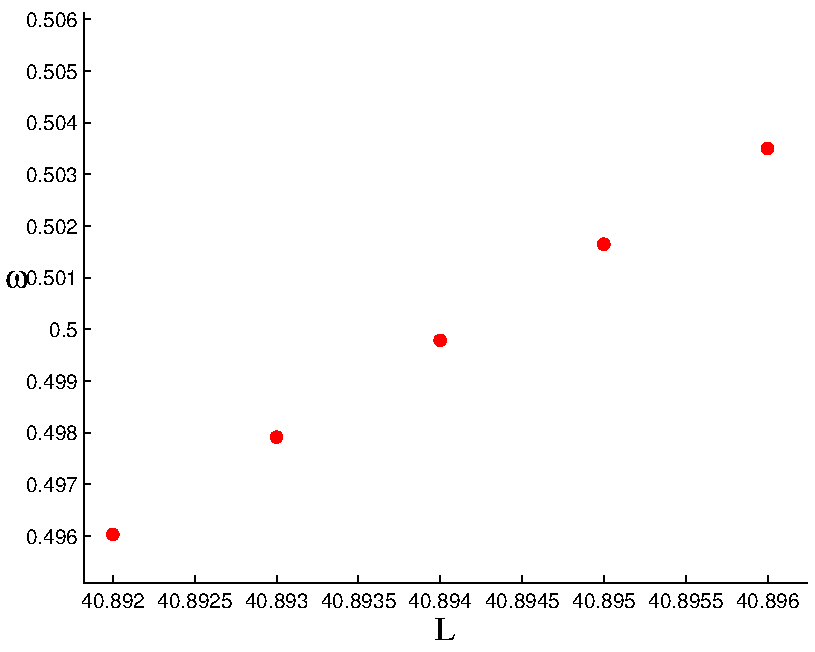
\includegraphics[width=0.45\textwidth]{KSZoomW}
 (b) 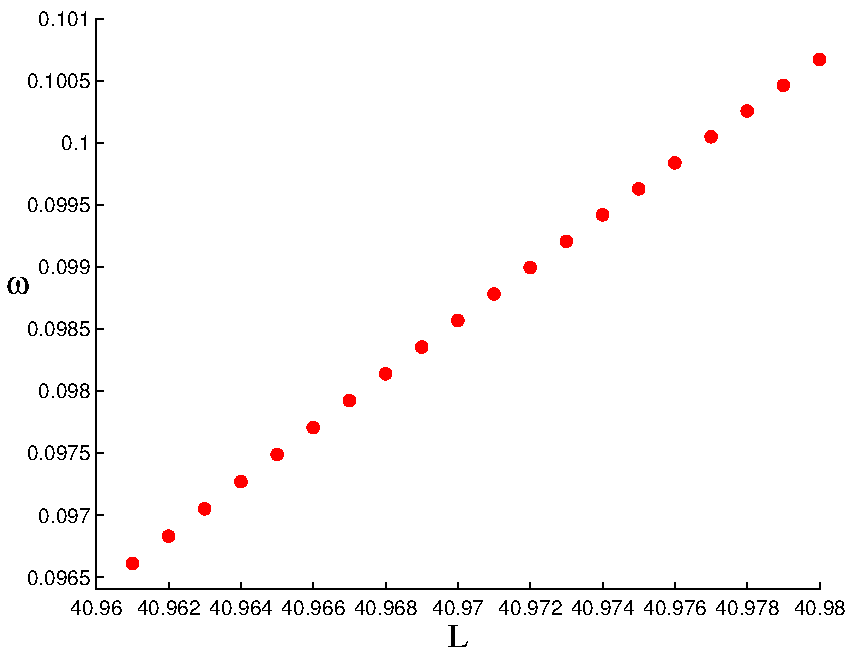
\includegraphics[width=0.45\textwidth]{KSZoomW2}
  \caption{
(a) Rotation number $\omega$ for a range of values of $L$;
no resonance expected in this range.
(b)    Rotation number $\omega$ for a range of values of
$L\in[40.96,40.98]$.
The abscissa is $\omega/2\pi$, and we are looking for
resonances at rational values $\omega/2\pi= P/Q$. At
current resolution, the neighborhood of $\omega/2\pi= 1/10$
indicates no resonance.
   }
  \label{fig:ZoomRotNum}
 \end{figure}
        }
\PCpost{2013-12-23, 2013-12-26}{
%Are you sure $\omega$ being rational means that the winding number is rational? That
%there are no factors of $\pi$'s and/or $L$'s involved? If you have the correct
%definition, $\omega$ should be an integer or a small-denominator rational
%for your \po.

According to \refeq{circMap} ${\bf x}(s)={\bf x}(s+2\pi)$, so the lowest
denominator rational shift would be $\omega = \pi$. In units of $2\pi$
your $\omega/2\pi \approx 0.1$, so appearing smooth at $\omega = 1/2$ in
\reffig{fig:ZoomRotNum} does not mean anything in terms of resonances:
perhaps the closest candidate for mode locking is $\omega/\pi \approx
1/5$, or $\omega = 0.628318$.
            }

\AFpost{2013-12-27}{
% You are correct about the rationality of the winding number - I had
% forgotten about the $2\pi$.
I took a closer look at $L\in[40.96,40.98]$,
see \reffig{fig:ZoomRotNum}\,(b) (I normalized the axes to make things clearer-I
will do the same for the poster)
    }

\AFpost{2013-12-22}{
My poster is split into 3 sections: Background of \KS, background of the Newton algorithm, and results.  For the results section I was planning on including a Poincar\'e section image, an image showing $\omega$ as a function of $L$ (and a small insert showing the magnified data), and then a third visualization of the quasi\po.  In point 3 above you mention that the coordinate axes should  physically important.  Can you elaborate on this a bit?  I read through \refref{SCD07} - there seem to be many ways to plot the data.  Were you thinking of a plot of $u(x,t)$ such as figure 2.1?  Or something like figure 5.6(a), where you plot an unstable manifold?

In response to some of your other questions: \\

 I can compute the torus for $L \in [40.81, 41.20]$, however when $L>41.18$ the ``torus'' has essentially collapsed onto the \po\ (if I plot it I get a point).  I'm not sure why the algorithm fails for $L<40.81$.  I will explore this tomorrow morning.  Hopefully I can find a way to resolve this.
            }

\PCpost{2013-12-24}{
 few general comments on the poster

\begin{enumerate}
  \item motivation?
  \item mention partially hyperbolic tori
  \item explain that you are working on a Poincar\'e return map rather
  than a flow
  \item Our research topic, between us, not for the poster: we
  know that working on the flow is better, at least for \po s.
  \item whether they play role comparable to / more important than
  equilibria and \po s?
\end{enumerate}
            }

\AFpost{2013-12-26}{
I'm looking for another way to visualize the tori.  I have a Poincar\'e
map image in the poster, but as you mentioned earlier, it would be nice
to show it in a more concrete way.
    }

\PCpost{2013-12-19, 2013-12-26}{
    It would be pedagogical for the DDaze poster gazers to actually plot
    at least one $2D$ torus projection - they will not appreciate that
    the Poincar'e section is a section of a hard-to find torus.
    The 3 projection coordinates \emph{should not} be some random
    Fourier modes (as in our early papers).

The coordinate axes should
    be constructed from physically important invariant solutions, as
    in ChaosBook.org/tutorials, see
\HREF{http://chaosbook.org/tutorials/halfcellshifts1.html} {here}.
    The method was introduced in Sect. 6. ``A tour of plane Couette state-space''
of \refref{GHCW07}
(click \HREF{http://www.cns.gatech.edu/~predrag/papers/preprints.html\#steady}
{here}).
\refRef{SCD07} is full of such visualizations; one choses as the origin
an important state, and as the two or three physical coordinate bases the
vectors connecting this solution to other solutions, or stability eigenvectors,
or whatever else is convenient. Further examples
are visualizations of \refref{ACHKW11}.
    }

\AFpost{2013-12-26}{
I'm not sure about your last point yet: do these tori play a comparable
/ more important role than \po s?  I would imagine they play a
more important role based on dimensionality, but as far as I know this
has never been shown (at least not in these systems).  Do you have any
particular insight here?
    }

\PCpost{2013-12-26}{
If we succeed populating the \statesp\ of \KS\ with a hierarchy of
partially hyperbolic tori, we would be the first to do it for any
dynamical system.
    }

\PCpost{2013-12-23, 2013-12-26}{
Lan has a torus at
$(L,\omega) = (40.95,0.5968)$, which you have verified, but the axes
in your \reffig{fig:Snorm}\,(a) should be labeled $(a_4,a_7)$, right?
}

\AFpost{2013-12-27}{
I did compute Lan's torus, however got a slightly different winding
number, $\omega=0.5913$.  The difference is small and I'm not concerned
by it.  The axes are correctly labeled - they are the same as Fig.~8\,(b)
in \refref{LCC06}.
    }


\AFpost{2013-12-27}{
For the visualization I've been playing around with two things.  First, I
liked figure 5.1 (d) from  \refref{SCD07}, so I tried to make a picture
like that. It ended up looking very boring, so I tried making a picture
like figure 4.1 instead, see \reffig{fig:UplotL4095}.  I'm not sure
how ``interesting'' this figure is- what do you think?
\begin{figure}[!h]
\centering
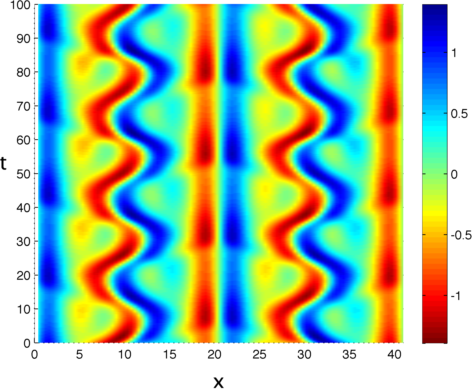
\includegraphics[width=3in]{UplotL4095}
  \caption{
   Color-coded $u(x,t)$ for the invariant torus, $L=40.95$.
   Horizontal; spatial position $x \in [0,L]$.
   Vertical: time $t$. As $u(x,t)$ belongs to the antisymmetric
subspace, it would suffice to plot $x \in [0,L/2]$.
   }
  \label{fig:UplotL4095}
 \end{figure}
    }

\PCpost{2013-12-28}{Fig.~5.1\,(d) from  \refref{SCD07}
was useful to us for \eqva\ and \reqva, I think it gets messy for
\po s. Your
\reffig{fig:UplotL4095} looks correct,
and is interesting to me, as it looks very much like
the dominant \po s for $L=38.5$, see fig.~1 in \refref{lanCvit07}.
Lan writes ``The Poincar\'e section return times are in the range
 $T=24.18 \pm 0.3$'', so could it be that Lan's torus arises
from a Hopf bifurcation of
one of the short orbits studied in \refref{lanCvit07}, continued
from $L = 38.5$ to $L=40.95$? In Table~II \po\ \cycle{01} with
$\period{01} = 25.6356$ looks like a natural candidate. It should
have a complex Floquet exponents, and the imaginary part should give
you a good estimate of the shift $\omega$ that you compute for
the torus.

That brings me back to the worries of {\bf 2013-12-22 Predrag} quoted
above: the variation of Fourier modes across the torus is minute, so it
could be that this is a Hopf bifurcation so close to the mother \po\
that nonlinear coupling of the two frequencies is so week that
mode-locking is negligible. In that case the quasiperiodic solution will
be so close to a \po\ that if you plot it in the full \statesp\ it
will be indistinguishable by naked eye from a \po.


BTW, as in this subspace $u(x,t)$ is antisymmetric, we always
plot only the $[0, L/2]$ interval.
    }

\AFpost{2013-12-26}{
My next step is to construct a figure like 5.4 (a) from  \refref{SCD07}.  Here they choose the axes $v_1$, $v_2$, and $v_3$ as projections onto three orthonormal vectors constructed from vectors Re ${\bf e}^{(1)}$, Im ${\bf e}^{(1)}$, and Re ${\bf e}^{(6)}$ via Gram-Schmidt.  I believe the ${\bf e}^{(j)}$ are the eigenvectors associated with the $j^{th}$ eigenvalue of the equilibria and relative equilibria of the \KS\ system.

I would expect do to something similar here - project the solution onto the eigenvectors of the stability matrix for the torus.   If we look at the first point at $L=40.95$ we find the stability matrix has a pair of complex roots with positive real part, a pair of complex roots with negative real part, three positive real roots, one negative real root, and 7 roots that are essentially zero.

My plan is to use the real and complex parts of the eigenvectors from the unstable complex eigenvalues, and perhaps the real eigenvector from stable complex eigenvalues.  Does that seem reasonable?

%When do you get back to Atlanta?  It'd be nice to sit down in person and
%talk a bit before Dynamics Days if you have the time.
%\\
%{\bf Predrag:} I return afternoon on Jan 1 - so Skyping before then would be more
%efficient.
    }

\PCpost{2013-12-28}{ Perhaps before constructing figures like
5.4\,(a) from  \refref{SCD07}, fig.~8.2 would be quick for you to plot,
and would give you a sense how `fat' the torus is in the full \statesp.
I suspect so thin to be indistinguishable by naked eye from a \po. If you
plot only the point on the Poincar\'e section, that will probably look
like an ellipse hugging the diagonal in the $(P,D)$ plot.
  }

\AFpost{2013-12-29}{
A few notes:
\begin{itemize}
% \item
% The abscissa in  \reffig{fig:ZoomRotNum} is $\omega/2\pi$.  I will use these same axes on my poster.
 \item
 I attempted to make a $(P,D)$ plot \reffig{fig:PvsD}
for $0 \leq t \leq 25$, but I'm not sure about my results.
I find both $P$ and
 $D$ to be very small, which seems problematic - I may simply be missing
 some scaling constant somewhere.  As you predicted, the points hug the
 diagonal (which I plotted in a black for reference).
 \begin{figure}[!h]
\centering
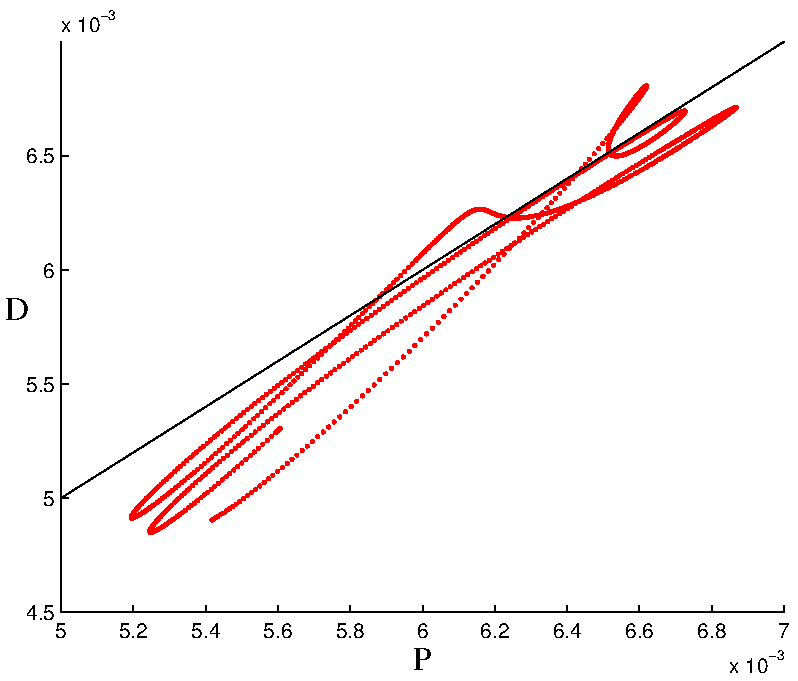
\includegraphics[width=3in]{PvsD}
  \caption{
   Power vs. Dissipation at $L=40.95$.
   }
  \label{fig:PvsD}
 \end{figure}

  \item
 I feel the need to focus on my poster for the next day or so.  I will include \reffig{fig:UplotL4095}, the tori on the Poincar\'e section, and the graph of $\omega/2\pi$ as a function of $L$.  I'll try to get a .pdf to you tomorrow to review.
 \item
 Skyping would be great if you have the time.  I emailed you my schedule, but I can move things around if needed.
 \end{itemize}
    }


\PCpost{2013-12-28}{
Moved all text that could be used in the forthcoming article into
\refchap{chap:KStori}. \refFig{fig:PvsD} does not look correct - I would
expect scales to be of order 1 (see Fig 8.1\,(a) in \refref{SCD07}).
These are points on the invariant torus, or is it a random trajectory?
Please read \refsect{sec:energy} {Energy transfer rates}.
    }

\AFpost{2013-12-30}{
Am I correct that
\[
    \expct{\obser} = \hat{a}_0
\,?
\]
That is-the zeroth Fourier Coefficient gives the spatial average?  To
generate \refFig{fig:PvsD} I took my Fourier Series for $u(x,t)$ (which
trivially means I have the Fourier series for $u_x$ and $u_{xx}$ and
generated 128 points in real space for both  $u_x$ and $u_{xx}$ at fixed
$t$.  I then squared these points, took the Fourier Transform, and
plotted the zeroth mode (divided by $L$ as per \refsect{sec:energy}).  I
repeated this process for $0 \leq t \leq 30$ to generate
\refFig{fig:PvsD}.  Am I mistaken?
    }

\PCpost{2013-12-30}{
In the Fourier
space the energy is a diagonalized quadratic norm \refeq{EFourier},
\beq
\expctE
          =  \sum_{k=-\infty}^{\infty} E_k
\,,\qquad
E_k(t) =
    {\textstyle\frac{1}{2}}|a_k(t)|^2
\,,
\ee{AF:EFourier}
    }
From \refeq{EnRate}
the power $P$ input and the energy dissipation rate $D$ are
\beq
      P(t) =  \expct{u_{x}{}^2}
        = \sum_{k=-\infty}^{\infty} q_k^2 E_k
                \,,\quad
      D(t) =  \expct{u_{xx}{}^2}
        = \sum_{k=-\infty}^{\infty} q_k^4 E_k
\,.
\ee{AF:EnRate}
There is no division by $L$ - Fourier transform took care of that.
To plot the Poincar\'e section \reffig{fig:Snorm}\,(a) projected on the
$[E,P,D]$ one evaluates $E_k$ at each Poincar\'e section point,
evaluates the sums and plots the corresponding point. It should be a loop -
would look better if you plot it as a curve than a set of dots.
To plot the full
\statesp\ torus, one starts at each point and plots the projection
of the trajectory onto $[E(t),P(t),D(t)]$
for $t$ up to the first return time. I suspect it will be so thin that
it will look like a \po.
Lan writes ``The Poincar\'e section return times are in the range
 $T=24.18 \pm 0.3$''.

Looking at  \reffig{fig:UplotL4095} I suspect that there is not much variation
in these averages, so $[P,D]$ is likely to hug the diagonal, and not vary
much.

\AFpost{2013-12-31}{
Ok-here is what I'm doing.

I take my 128 points on the Poincar\'e section (each 16 dimensional, but we really know 32 dimensions since $a_{-k}=-a_k$) and compute the sums
\begin{align}
E=&\sum_{k=-16}^{16}E_k=\sum_{k=-16}^{16}\tfrac{1}{2}a_k^2=\sum_{k=1}^{16}a_k^2\\
P=&\sum_{k=1}^{16}q_k^2E_k=\sum_{k=1}^{16}(\frac{2\pi k}{L})^2a_k^2\\
D=&\sum_{k=1}^{16}q_k^4E_k=\sum_{k=1}^{16}(\frac{2\pi k}{L})^4a_k^2
\end{align}
at each point.  This gives me 128 values of $E$, $P$, and $D$.  Here is the plot below:
 \begin{figure}[!h]
\centering
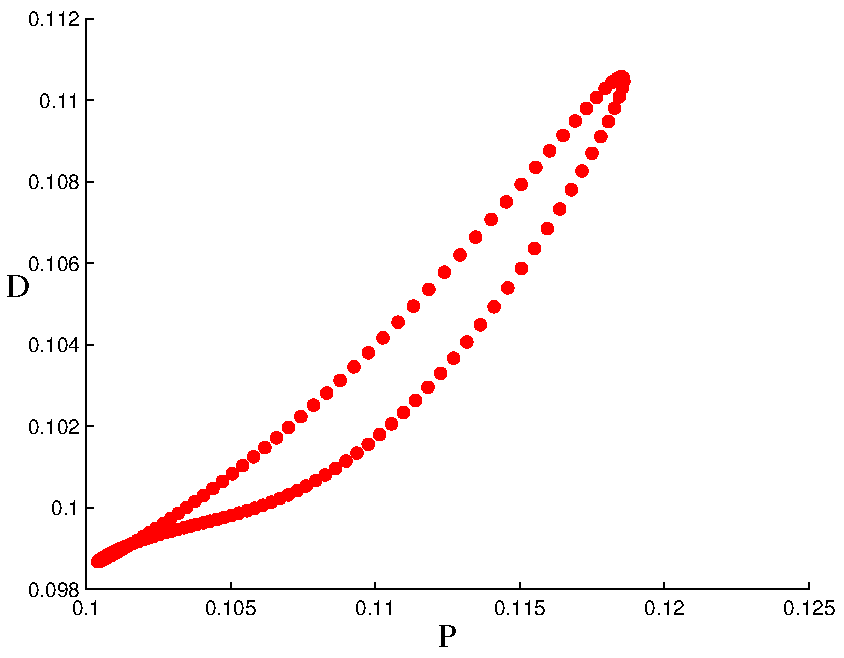
\includegraphics[width=3in]{PDplot2}
  \caption{
   Poincar\'e section: Power vs. dissipation at $L=40.95$.
   }
  \label{fig:PDplot2}
 \end{figure}

Now, doing this for the full state space is a bit tricky.  Every point on the Poincar\'e section has its own return time.  As an initial experiment I plotted the full state space torus for $t<25$ (slightly larger than one full return time). It looks somewhat odd and ``flat'' (although maybe that's the point?)  Here are several projections.

Do these plots seems correct to you?
 \begin{figure}[!h]
\centering
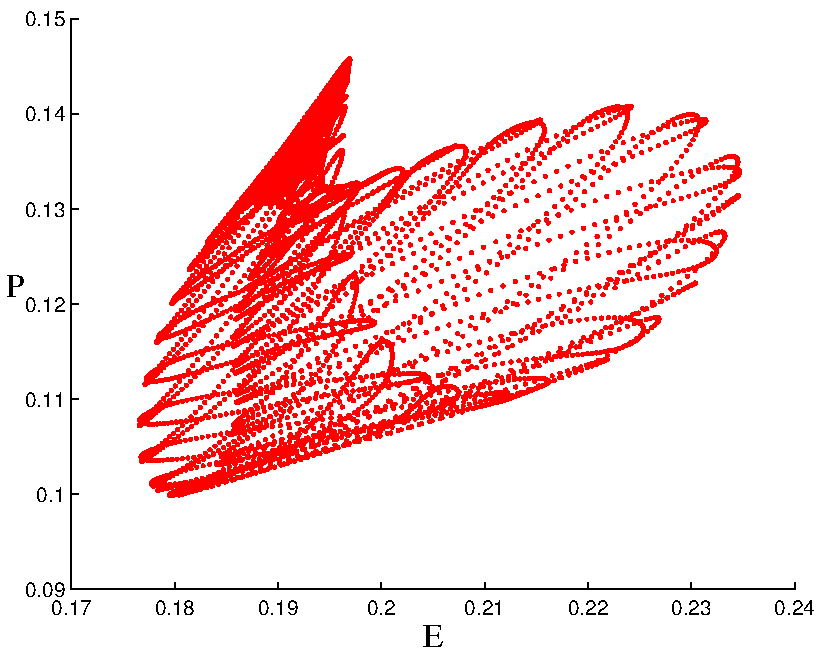
\includegraphics[width=3in]{FullEPD1}
  \caption{
   Energy vs. power at $L=40.95$.
   }
  \label{fig:FullEPD1}
 \end{figure}

\begin{figure}[!h]
\centering
 (a) 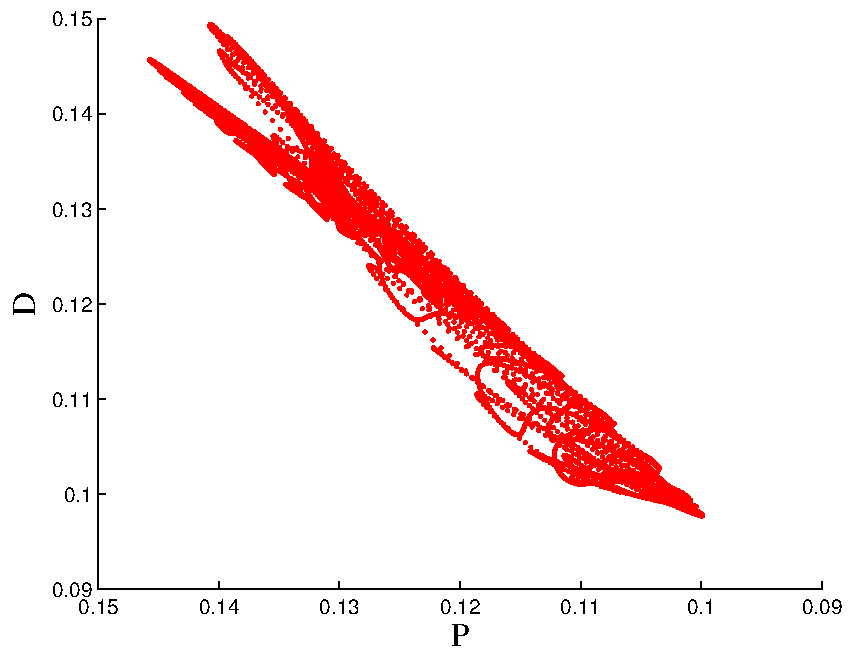
\includegraphics[width=0.45\textwidth]{FullEPD2}
 (b) 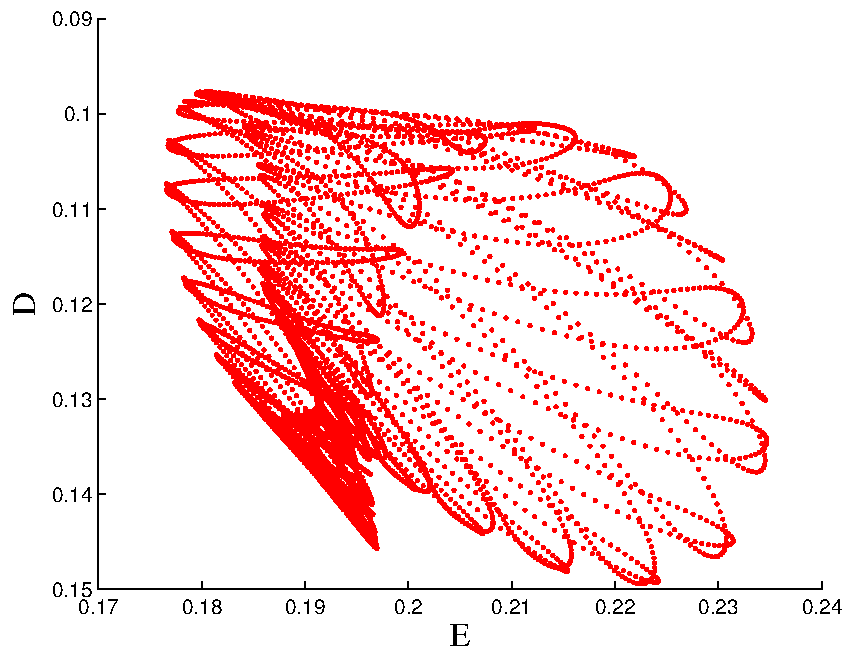
\includegraphics[width=0.45\textwidth]{FullEPD3}
  \caption{
   Full \statesp: (a) Power vs. dissipation at $L=40.95$
    (b) Energy vs. dissipation.
   }
  \label{fig:FullEPD2}
 \end{figure}

}

\PCpost{2013-12-31}{
The scale looks suspicious to me: I would expect scales to be of order 1
(see Fig 8.1\,(a) in \refref{SCD07}). In \reffig{fig:UplotL4095} $u(x,t)$
peaks at about $\pm 1$, I'm surprised that it's magnitude integrated over
the interval would be only $\approx 0.1$. Things are also further away
from the diagonal than what I would have expected. \refFig{fig:FullEPD1}
and \reffig{fig:FullEPD2} I cannot make any sense at all :)

    }

\AFpost{2014-1-9}{
Ok-  I'll keep thinking about the energy projections.

In the meantime, I will begin to explore the possibility that these orbits arise from a Hopf bifurcation of a \po. As we can see in \refFig{fig:PsecTorus} the modes seem to collapse near $L=40.25$ so it seems reasonable that the \po\ is located here.  I will attempt to compute it, then study its spectrum and see if I can detect a Hopf bifurcation.

Is the method in \refref{lanVar1} the best for computing these orbits?
 }

\AFpost{2014-1-9}{
{\bf Notes from meeting on 1/13: }\\

I will implement the \po\ find described in \refref{lanVar1} and study the spectrum of these \po s to determine if the torus we found arose from a Hopf bifurcation.  I will further verify that the rotation number of the \po\ is similar to the rotation number of the torus.  If this is the case I will see if I can find other tori near other \po s.  Hopefully we can establish that this behavior is generic.

Ideally we will find a large torus that covers a large area of space.  We can then study the impact this torus has on the global dynamics.
 }

 \AFpost{2014-1-26}{

I am currently working on the \po\ finder described in \refref{lanVar1}.  I believe I have a good understanding of it, however wanted to clarify one things.

In Equation (18) of \refref{lanVar1} the $Nd$ dimensional vector $\hat{a}$ is said to ``impose the constraint on the coordinate variations $\delta\hat{x}$.''  I believe this constraint (at least in the \KSe\ case) is that we fix the first point of the discretization (so $a_1(s_1,\tau)=\mbox{const.}$).  In my case, this would be the Poincar\'e section $a_1=0.06$.  Is this correct? So essentially in my case $\hat{a}=(1,0,0\cdots,0)$?


 }

 \AFpost{2014-1-28}{

The \po\ finder is working well.  I used one point of the quasi\po\ for $L=41.2$ as an initial guess for the algorithm.  As we can see in \refFig{fig:PsecTorus}, the quasi\po\ varies very little, implying that it is very close to the \po\ (assuming one exists).  The algorithm successfully converged to an error less than $10^{-14}$.  The \po\ is shown below.  It has a period $T \approx24.1107$.

 \begin{figure}[!h]
\centering
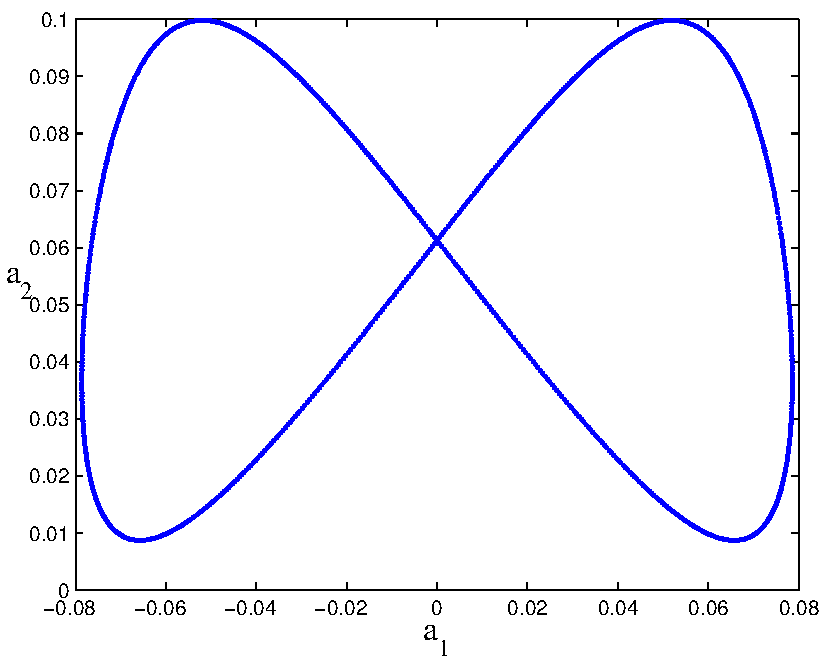
\includegraphics[width=3in]{POrbit1}
  \caption{
   \Po\ at $L=41.2$ with period $T \approx24.1107$.
   }
  \label{fig:POrbit1}
 \end{figure}

I then began to change $L$ and monitored the eigenvalues of the Jacobian of the matrix.  These are shown in \refFig{fig:POrbitEig}.  The eigenvalues are purely imaginary near $L\approx 41.95$.  It seems reasonable to conjecture that the torus is created at this point through a Hopf bifurcation.  At $L \approx 40.8$ the complex conjugate eigenvalues collide and become real.  This corresponds to the point where the quasi\po\ finder fails.

The existence of the torus can therefore be established by studying the eigenvalues of the nearby \po.  My goal is to inspect several other \po s to determine if this sort of behavior is typical.  Do you have any suggestions for which orbits?  I cannot find the repository that you mentioned - can you please remind me the name?

\begin{figure}[!h]
\centering
 (a) 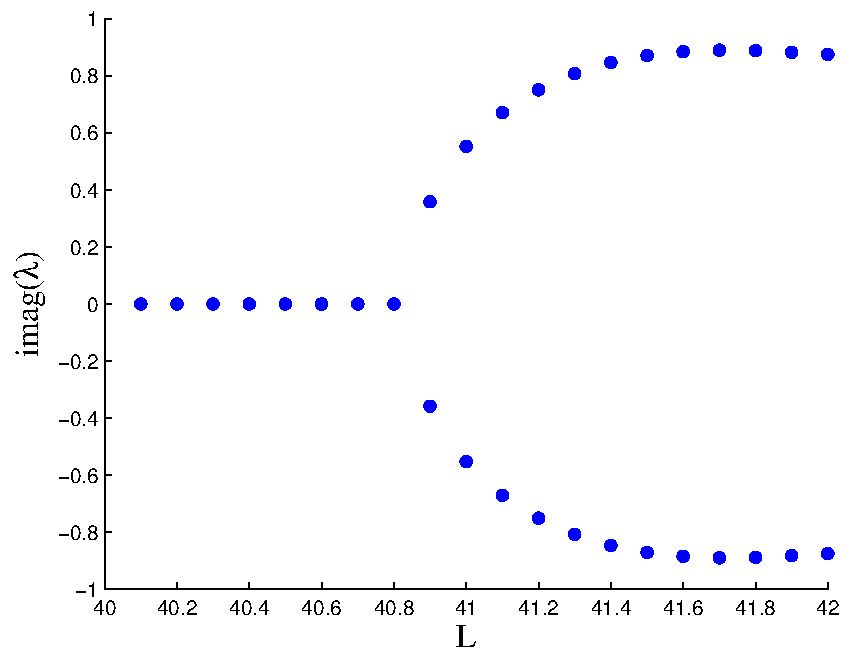
\includegraphics[width=0.45\textwidth]{LVImagEig}
 (b) 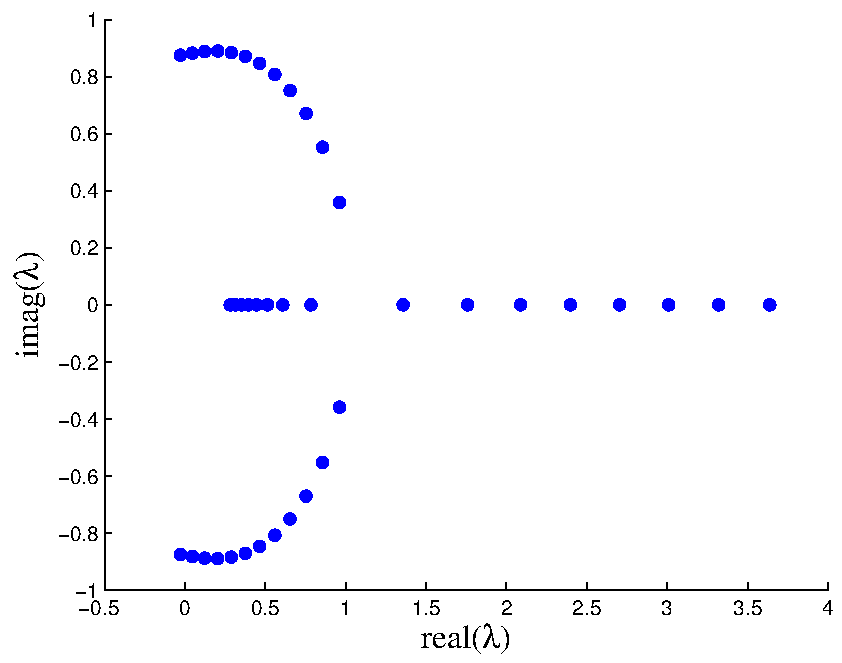
\includegraphics[width=0.45\textwidth]{RealVImagEig}
  \caption{
  (a) Imaginary part of eigenvalues as a function of the parameter $L$
    (b) Imaginary part of eigenvalues as a function of the real part.
   }
  \label{fig:POrbitEig}
 \end{figure}

 }

  \AFpost{2014-5-28}{

After a 4 month hiatus....

I've begun looking at the \po s and tori again.  I ran a little toy experiment to try to understand the dynamics a bit better.  I began with $L=40.85$.  In the figure below I plotted the a torus and \po\ (both in black) and three randomly chosen orbits in the same neighborhood.  As we can see these orbits (red, green, and blue) are all attracted to the torus, and remain near the torus, at least for moderate amounts of time (I looked at about 300 returns).  This applied to both orbits within the torus (red and green) and without (cyan).

 \begin{figure}[!h]
\centering
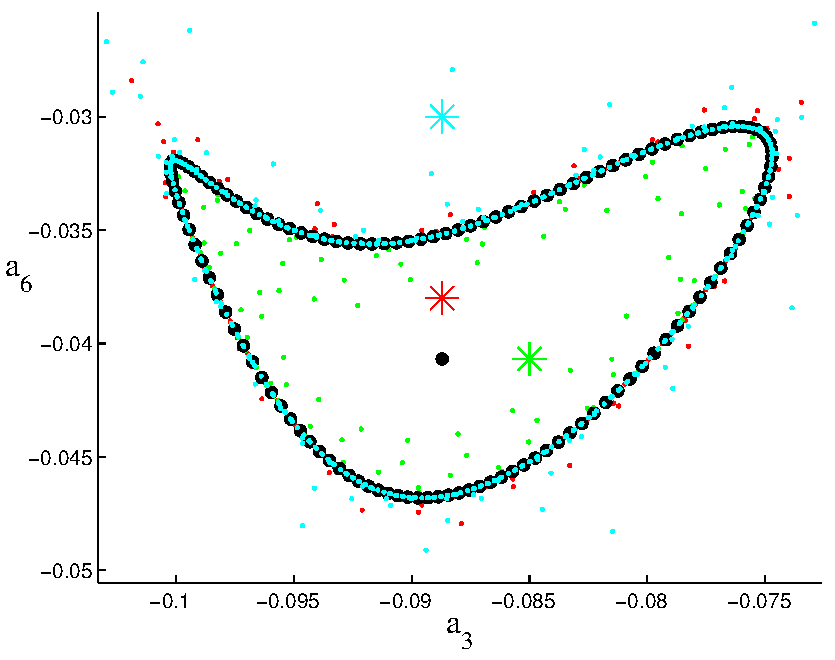
\includegraphics[width=3in]{L_40p85}
  \caption{
   \Po\ at $L=41.2$ with period $T \approx24.1107$.
   }
  \label{fig:RandOrbs}
 \end{figure}

I repeated this experiment for values of $L$ for which there was no torus - both before the Hopf bifurcation and after the torus is destroyed.

In the figure to the right we see $L=42$, prior to the Hopf bifurcation.  In this case we can see the orbit being attracted and repelled from the \po.  It gives a nice visualization of the stable and unstable manifolds (I think).

In the \PCedit{right} figure we see $L=40$, after the torus has been
destroyed.  The black dot indicates the \po\ and the red star
is the random orbit's initial point.  Here we can see the orbit is
attracted to a different \po.  I will discuss this orbit
below.

\begin{figure}[!h]
\centering
 (a) 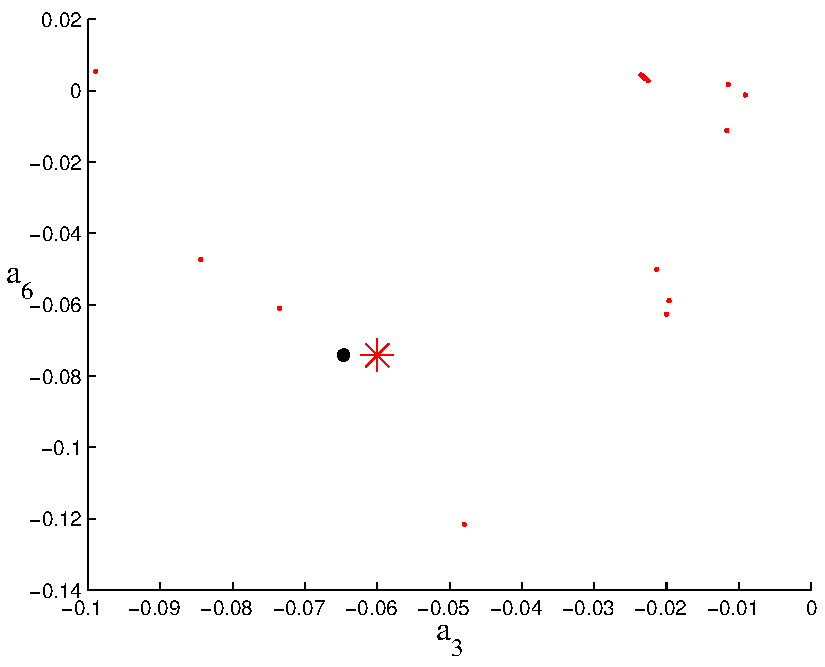
\includegraphics[width=0.45\textwidth]{L_40}
 (b) 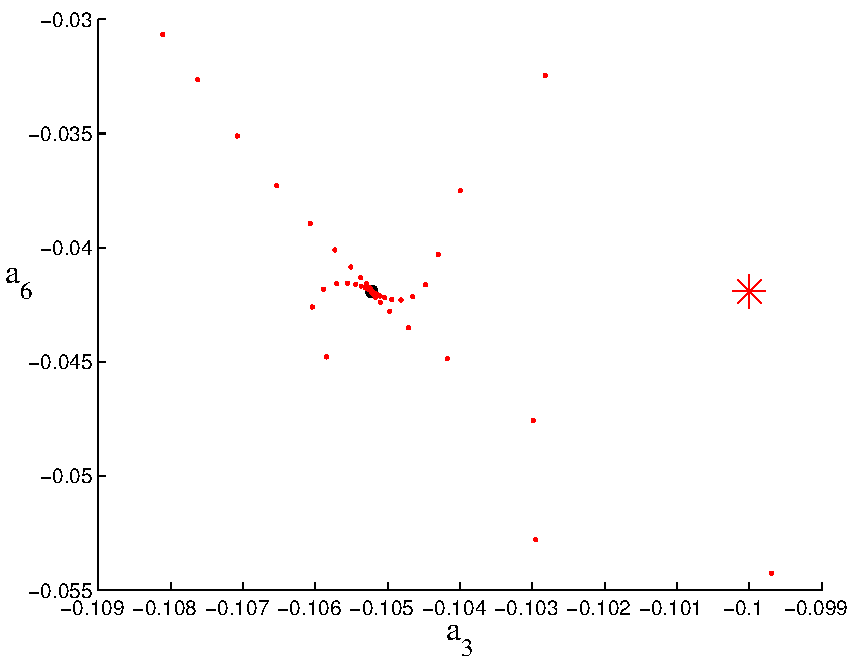
\includegraphics[width=0.45\textwidth]{L_42}
  \caption{
  Poincar\'e section at (a) $L=40$;
    (b) $L=42$.
   }
  \label{fig:BeforeAfterTorus}
 \end{figure}


Another interesting point.  I messed up my first run at $L=42$ and chose an initial point for the orbit far from the \po.  The result is shown below.  Here we see the orbit following some sort of structure.  I iterated this orbit thousands of times, however I kept getting the same image.  I'm not sure what this is.  It isn't closed as I would expect a torus to be.  Thoughts?

 \begin{figure}[!h]
\centering
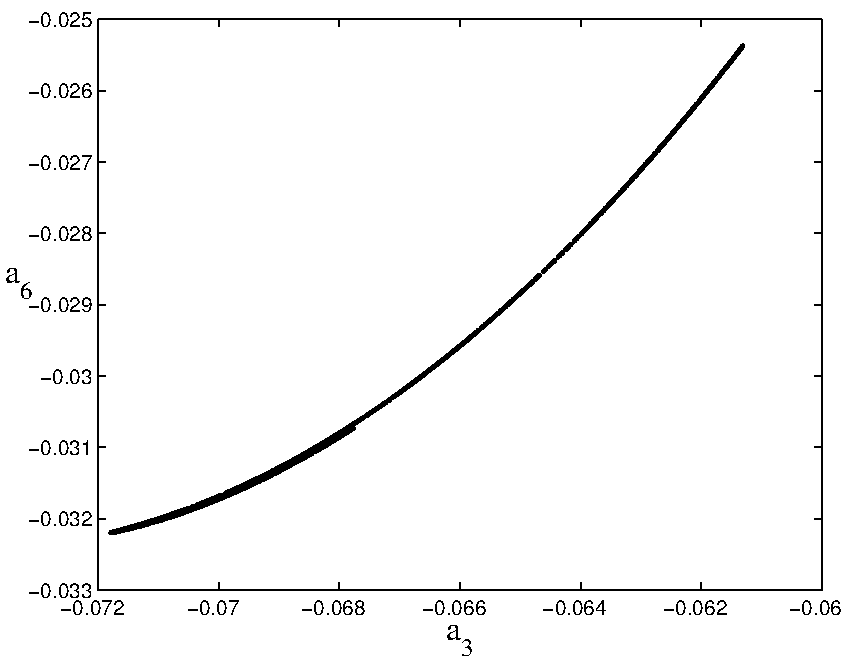
\includegraphics[width=3in]{OddThing}
  \caption{
   \Po\ at $L=41.2$ with period $T \approx24.1107$.
   }
  \label{fig:WeirdThing}
 \end{figure}

As I mentioned above I found a new \po\ at $L=40$.  I tracked this orbit throughout parameter space hoping to find a Hopf bifurcation.  Unfortunately I did not see one.  The dominant eigenvalues are never complex.  I also hoped that this might be a period-doubled orbit after the destruction of Lan's torus.  However, I was unable to compute this second \po\ for values of $L$ near where the torus is destroyed.  Furthermore, when they two \po s do coexist, their periods do not appear to be rationally related.  For example, at $L=40.3$ the periods are 24.1517 for Lan's orbit and 55.0812 for the other.

However - this got me thinking that this method could be used to detect the creation of a new \po\ when the torus is destroyed.  I looked at the Poincar\'e section with $L=40.8$, soon after the torus is destroyed.  I saw the left picture below.  The orbit seems to accumulate near a new point (which I've plotted as a black star).  I hypothesized that this was a new \po\ and found that it indeed was.

\begin{figure}[!h]
\centering
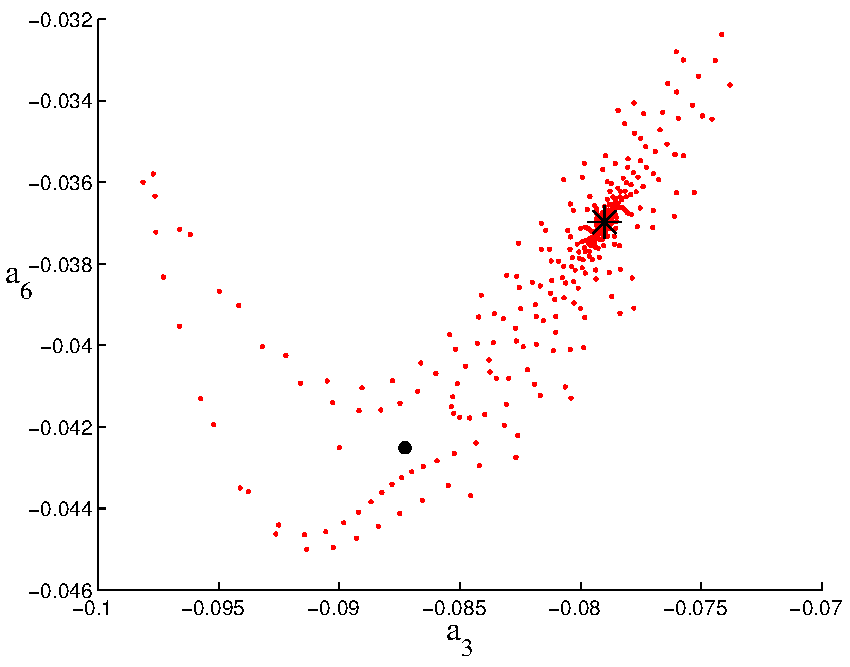
\includegraphics[width=3in]{L40p8}
  \caption{
   Poincar\'e section at $L=40.8$.  The Lan \po\ is shown with a black dot.  The new \po\ is shown with a black star.
   }
  \label{fig:L40p8}
 \end{figure}

I tracked this \po\ in parameter space and found that it was created at approximately $L=40.835$.   Unfortunately, the torus still exists here.  The creation of this \po\ may therefore not be related to the torus.  Further study is needed.

 \begin{figure}[!h]
\centering
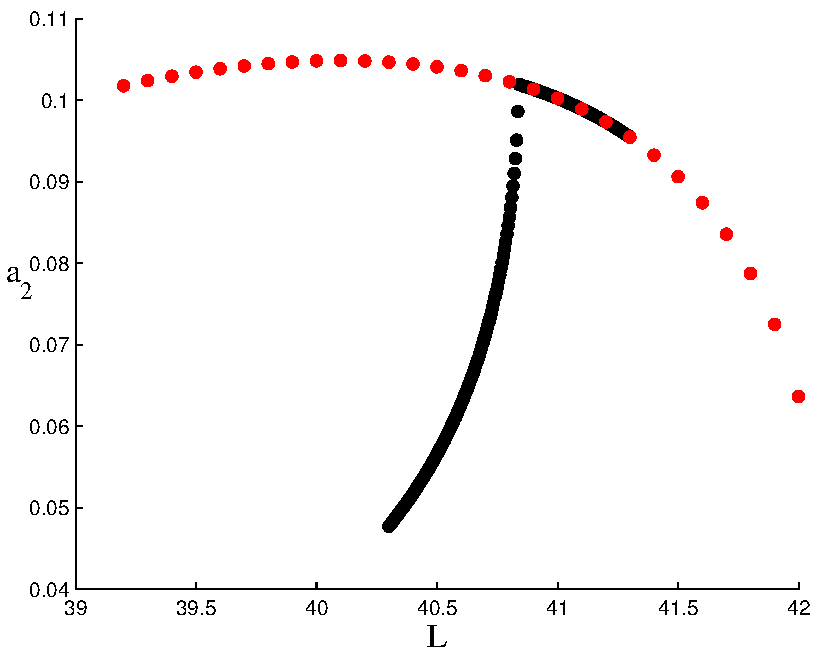
\includegraphics[width=3in]{Bifurcation}
  \caption{
   Initial $a_2$ coordinate of the Lan \po\ (red) and new \po\ (black).
   }
  \label{fig:Bifurcation}
 \end{figure}
 }

   \AFpost{2014-5-29}{

Ok-upon closer examination it appears that the creation of the new \po\ (see previous notes) does indeed occur at the same time the eigenvalues of Lan's \po\ collide on the real line.  HOWEVER - the torus persists beyond this point!
To Review:
\begin{enumerate}
\item Hopf Bifurcation creates torus at $L \approx 42$.
\item Complex Eigenvalues of original \po\ collide at $L \approx 40.84$.  New \po s created with same period.
\item Torus disappears around $L=40.8$
\end{enumerate}
So...why does the torus disappear?  And what, if anything, replaces it?

There doesn't appear to be anything significant with the eigenvalues of either \po.  Note: The new \po\ appears to undergo a Hopf bifurcation near $L=40.5275$.  Maybe look for a torus here?

To do: \\
Iterate end of bottom fold lots of times.  window: -0.0681 to -0.0676, -0.0309, -0.0305\\
For Figure 6.12 plot dominant eigenvectors \\
How do you hop around in Fig 6.12b

 }

\AFpost{2014-06-02}{ {\bf Summary: The Life and Death of an Invariant
torus in the \KSe\ }
\\
{\bf [Predrag 2014-06-14]} moved this text to \texttt{FoxCvi14.tex} .

 Another interesting fact - these tori do not always arise from Hopf bifurcations.  For example, the \po\ generated by the bifurcation at $L \approx 40.84$ undergoes a Hopf-like birfucation at $L\approx 40.53$.  I examined the region around this \po\ for a torus yet could not find one.  I am somewhat surprised by this - I would expect that this bifurcation would result in the same behavior.  So-why do we get a torus in one case but not the other?

 One possible explanation - both orbits have a single multiplier of 1 and a complex pair.  When the torus exists the next largest multiplier is order $10^{-2}$.  When there is no torus the next largest multiplier is an order of magnitude smaller $10^{-3}$.    In both cases they are positive.

 Finally - I think it would be really helpful to have some idea of what we want the first real paper to contain.  It seems there is a lot of interesting stuff - we have the tori, the bifurcations of \po s, etc.  Do we want to focus on one thing in particular or cover all of it?  I suppose the paper could focus on bifurcations of \po s, and we could simply discuss the tori as the result of one such bifurcation.  What do you think?
 }

\AFpost{2014-4-02}{
I've been tracking \po\ s in the region of phase space we've been looking at.  Here is a cute little picture.

The orbit on the bottom just seems to be hanging out.  I can't continue it to any of the other orbits.  Not sure if its separate, or just difficult to compute near the bifurcation points.
 \begin{figure}[!h]
\centering
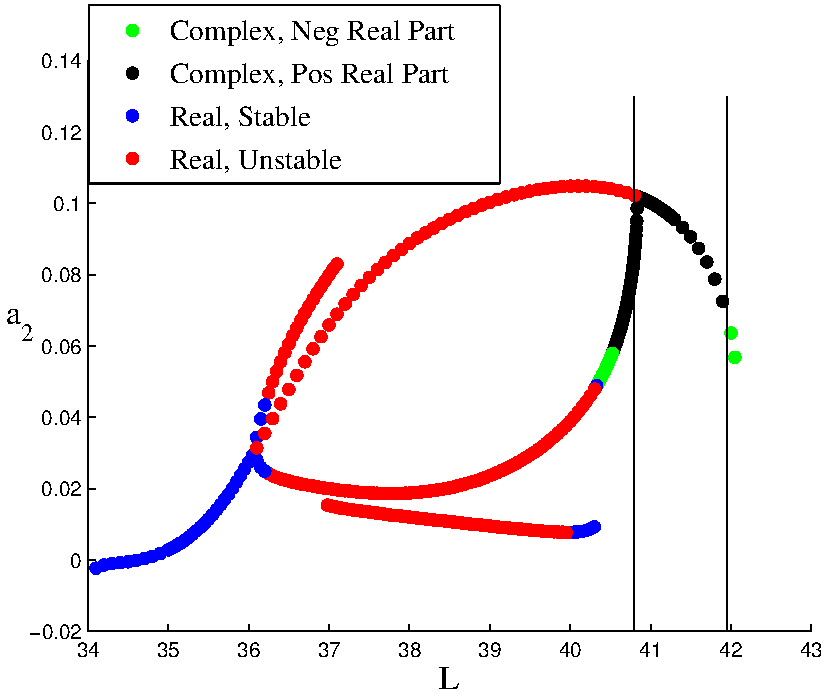
\includegraphics[width=3in]{PeriodicOrbitsStab}
  \caption{
  The $a_2$ initial conditions for \po s.  The stability is indicated by the color.  The torus only exists between the black lines.
   }
  \label{fig:StabPlot}
 \end{figure}
 }

    \PCpost{2014-06-09}{
A preprint of possible interest\rf{LROBK13} has revised version on the archive,
\HREF{http://www.comp-phys.tu-dresden.de/supp/} {videos} of 3D phase-space
  slices.
    }

\AFpost{2015-04-23}{ I'm running into a problem and thought you might
have some insight.  I'm trying to compute tubes (like in the KS System)
for the Circular Restricted 3 body problem.  We know these tubes exist,
but the variational algorithm keeps converging to the periodic orbit in
the center of the tube.  Although this solutions is valid it is
trivial.  Any thoughts on how to avoid this?
        }

\NBBpost{2015-06-17}{
    I have a general question though: Are these tori unstable? Because
    you say that the initial torus that is born from the bifurcation is
    stable, and if that is also the case for the larger ones, isn't the
    variational method is somewhat an overkill to detect them?
    }

\AFpost{2015-06-18}{
Perhaps overkill, but I like using a similar method for both the periodic
orbits and tori.

It's also possible that some tori may be unstable so I think its nice
that we present a method that will work for all of them.
    }

\AFpost{2015-06-18}{
I'm adding a bit more to explain why we do a cutoff at N=16 modes.  It
seems this was first done/justified in Spatiotemporal chaos in terms of
recurrent patterns.  They use L values around 36, a bit lower than our
40-42.
Do you think these parameters are close enough that we can use this to
    justify our choice of truncation to 16?
    }
\PCpost{2015-09-26}{
I am comfortable with 16 modes for this calculation
    }

    \PCpost{2015-09-15}{ Reading about robustness of invariant tori.
Farazmand likes to refer to Fenichel\rf{Feniche71} (I should put a copy
\HREF{http://chaosbook.org/library/Feniche71.pdf}{here}). My
understanding is that if a stability exponent is purely imaginary, it
can destroy a torus at an rational resonance; but if it has a real part
(hyperbolic case), there is no way for the Floquet exponent to approach
the purely imaginary winding number of the torus, there can be no
resonance, and the torus remains smooth and robust for an open interval
of the system parameter values.

Figueras and Haro\rf{FigHar12} write:
``it has been known for a long time that persistence of invariant
manifolds is closely related to the concept of normal
hyperbolicity\rf{Feniche71}. %21
%34 M. W. Hirsch, C. C. Pugh, and M. Shub, Invariant manifolds,
%    Lecture Notes in Math. 583, Springer-Verlag, Berlin, 1977.
%50 R. Ma\~{n}\'e, Persistent manifolds are normally hyperbolic,
%   Trans. Amer. Math. Soc., 246 (1978), pp. 261–283.
%57 R. J. Sacker, A new approach to the perturbation theory of
%    invariant surfaces, Comm. Pure Appl. Math., 18 (1965), pp. 717–732.
We consider the analogous
concept, tailored for skew products over rotations. Roughly speaking, an
invariant torus is fiberwise hyperbolic if the linearized dynamics on the
normal bundle is exponentially dichotomous, that is, the normal bundle
splits into stable and unstable bundles on which the dynamics is
uniformly contracting and expanding, respectively. Notice that the
tangent dynamics is dominated by the normal dynamics, since the former
presents zero Lyapunov exponents. This implies that fiberwise hyperbolic
invariant tori are robust and are as smooth as the system [ 28 ].
% A. Haro and R. de la Llave, A parameterization method for the
% computation of invariant tori and their whiskers in quasi-periodic maps:
% Rigorous results, J. Differential Equations, 228 (2006), pp. 530–579.
''

Figueras' thesis might be an easier read:
\HREF{http://www2.math.uu.se/~figueras/preprints/files/phd_thesis/Jordi_LLuis_Figueras_Romero_PHD.pdf}
{click here}.
    }

    \PCpost{2015-09-26}{
to Adam: I've been holding up FoxCvi14 paper\rf{FoxCvi14} for way too long,
and you have a November deadline at your University, so I've removed myself as
a co-author, and you go ahead with fixing small things (that we have discussed
in the Skype) and ship it off to \texttt{arXiv} pronto. Do not rename the files
from \texttt{FoxCvi14}, that screws up zillion cross links between different svn
repositories:)
    }

\end{description}
